\begin{thm}{079}{\hosi 3}{}
 相異なる実数$x, y$に関して、$2^x+4^y=4^x+2^y$ が成り立っているとき、$8^x+8^y+6$ の取りうる値の範囲を求めよ。
\end{thm}

$2^x=X$, $2^y=Y$とおくと、与式は$X-X^2=Y-Y^2$とかける。この値を$t$とおくと、方程式$x-x^2=t$は異なる2つの正の実数解$(X, Y)$を持つことが必要である。また解と係数の関係より、$X+Y=1$, $XY=t$である。

\begin{figure}[H]
 \centering
 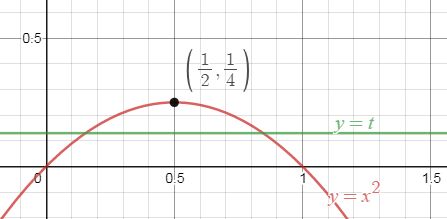
\includegraphics[width=0.7\linewidth]{../problems/Q_079/A_079.png}
\end{figure}
上図のように、$xy$平面において曲線$y=x-x^2$と直線$y=t$が、$x>0$の領域で2回交わればよいので、$0<t<\dfrac{1}{4}$となる。
\begin{align*}
 &8^x+8^y+6=X^3+Y^3+6 \\
 =&(X+Y)\bigl[(X+Y)^2-3XY\bigr]+6=7-3t
\end{align*}
であるから、
\[ \frac{25}{4}<8^x+8^y+6<7 \]